\documentclass{article}
\usepackage[utf8]{inputenc}

\title{Informe TL}
\date{April 2015}

\usepackage{natbib}
\usepackage{graphicx}
\usepackage{caratula}
\usepackage[spanish]{babel}


\begin{document}


%%%%%%%%%%%%%%%%%%%%%%%%%%%
%			INICIO DE CARÁTULA			%
%%%%%%%%%%%%%%%%%%%%%%%%%%%

%% **************************************************************************
%
%  Package 'caratula', version 0.2 (para componer caratulas de TPs del DC).
%
%  En caso de dudas, problemas o sugerencias sobre este package escribir a
%  Nico Rosner (nrosner arroba dc.uba.ar).
%
% **************************************************************************



% ----- Informacion sobre el package para el sistema -----------------------

\NeedsTeXFormat{LaTeX2e}
\ProvidesPackage{caratula}[2003/4/13 v0.1 Para componer caratulas de TPs del DC]


% ----- Imprimir un mensajito al procesar un .tex que use este package -----

\typeout{Cargando package 'caratula' v0.2 (21/4/2003)}


% ----- Algunas variables --------------------------------------------------

\let\Materia\relax
\let\Submateria\relax
\let\Titulo\relax
\let\Subtitulo\relax
\let\Grupo\relax


% ----- Comandos para que el usuario defina las variables ------------------

\def\materia#1{\def\Materia{#1}}
\def\submateria#1{\def\Submateria{#1}}
\def\titulo#1{\def\Titulo{#1}}
\def\subtitulo#1{\def\Subtitulo{#1}}
\def\grupo#1{\def\Grupo{#1}}


% ----- Token list para los integrantes ------------------------------------

\newtoks\intlist\intlist={}


% ----- Comando para que el usuario agregue integrantes

\def\integrante#1#2#3{\intlist=\expandafter{\the\intlist
	\rule{0pt}{1.2em}#1&#2&\tt #3\\[0.2em]}}


% ----- Macro para generar la tabla de integrantes -------------------------

\def\tablaints{%
	\begin{tabular}{|l@{\hspace{4ex}}c@{\hspace{4ex}}l|}
		\hline
		\rule{0pt}{1.2em}Integrante & LU & Correo electr\'onico\\[0.2em]
		\hline
		\the\intlist
		\hline
	\end{tabular}}


% ----- Codigo para manejo de errores --------------------------------------

\def\se{\let\ifsetuperror\iftrue}
\def\ifsetuperror{%
	\let\ifsetuperror\iffalse
	\ifx\Materia\relax\se\errhelp={Te olvidaste de proveer una \materia{}.}\fi
	\ifx\Titulo\relax\se\errhelp={Te olvidaste de proveer un \titulo{}.}\fi
	\edef\mlist{\the\intlist}\ifx\mlist\empty\se%
	\errhelp={Tenes que proveer al menos un \integrante{nombre}{lu}{email}.}\fi
	\expandafter\ifsetuperror}


% ----- Reemplazamos el comando \maketitle de LaTeX con el nuestro ---------

\def\maketitle{%
	\ifsetuperror\errmessage{Faltan datos de la caratula! Ingresar 'h' para mas informacion.}\fi
	\thispagestyle{empty}
	\begin{center}
	\vspace*{\stretch{2}}
	{\LARGE\textbf{\Materia}}\\[1em]
	\ifx\Submateria\relax\else{\Large \Submateria}\\[0.5em]\fi
	\par\vspace{\stretch{1}}
	{\large Departamento de Computaci\'on}\\[0.5em]
	{\large Facultad de Ciencias Exactas y Naturales}\\[0.5em]
	{\large Universidad de Buenos Aires}
	\par\vspace{\stretch{3}}
	{\Large \textbf{\Titulo}}\\[0.8em]
	{\Large \Subtitulo}
	\par\vspace{\stretch{3}}
	\ifx\Grupo\relax\else\textbf{\Grupo}\par\bigskip\fi
	\tablaints
	\end{center}
	\vspace*{\stretch{3}}
	\newpage}




\materia{Teor\'ia de Lenguajes}
\submateria{Primer Cuatrimestre de 2015}
\titulo{Recuperatorio Trabajo Práctico 1}

\grupo{Grupo Estado Final}
\integrante{Gorojovsky, Román}{530/02}{rgorojovsky@gmail.com}
\integrante{Lazzaro, Leonardo}{147/05}{lazzaroleonardo@gmail.com}
\integrante{Montero, Victor}{707/98}{vmontero@dc.uba.ar}

\begin{titlepage}
\maketitle
\thispagestyle{empty}
\end{titlepage} 

\newcommand{\Hopcroft}{\emph{Introduction to Automata Theory...} \citep{hopcroft}}

%%%%%%%%%%%%%%%%%%%%%%%%%%%
%				FIN DE CARÁTULA			%
%%%%%%%%%%%%%%%%%%%%%%%%%%%

%
\section{Reentrega}

Para le re-entrega se decidio mejorar el codigo en general.

\section*{Parser de RegEx}

Para parsear las expresiones regulares, se arma un \'arbol donde cada nodo corresponde a un a un operador o s\'imbolo.

Este arbol se arma recurvisamente mientras se lee la entrada.

Cada operador o simbolo tiene si propia clase y esta clase
implementa la conversion a un automata.
La forma de convertir el automata sigue conservando la idea de la entrega original, salvo que ahora cada Nodo encapsula esta conversion en el metodo "to_automata".

\section{Transiciones LAMBDA}

Para el problema de las transiciones LAMBDA, la clase automata implementa correctamente el metodo "is_deterministic" considerando el caso cuando hay una transicion LAMBDA.
Ademas, en los simbolos del automata no permitimos la existencia del LAMBDA. 


El algoritmo de minimizacion fue re-implmentado completamente y como entrada require un automata deterministico.
Ademas, este nuevo algoritmo nunca considera que se pueden tener transiciones LAMBDA.

\section{Ejercicio interseccion de automatas}

Se adapto el algoritmo para aceptar automatas con distinto conjuntos de simbolos.

\section{Correciones Menores}

Se aceptan automatas sin transiciones.
Se aceptan automatas sin estados finales
Se aceptan automatas sin estados finales, ni transiciones.

\section*{Organización general del código.}
El trabajo se realizó en \emph{Python}.  Se crearon tres módulos: \texttt{models} contiene la representación del autómata (clases \texttt{Automata} y \texttt{Node}), \texttt{parsers}  contiene funciones para leer los archivos según los formatos definidos (regex y autómata) y convertirlos en objetos de clase \texttt{Automata}, y \texttt{writers} contiene funciones que escriben objetos de dicha clase en formato de texto o \texttt{DOT}.  

Usando estas clases, se resolvieron los ejercicios en los archivos correspondientes, según el esqueleto provisto por la cátedra.  Para cada ejercicio se implemento un breve unit test en \texttt{test/test\_ejercicio\_x}.  También se implementaron unit tests para \texttt{models} y \texttt{parsers}.  En algunos casos hay también un script \texttt{run\_and\_plot\_ejercicio\_x} que ejecuta el ejercicio y presenta gráficamente el resultado.

\section*{Clase \texttt{Automata}}
La clase \texttt{Automata} contiene la lista de estados, los símbolos, el estado inicial y el
conjunto de finales.  Además tiene algunas funciones necesarias para resolver algunos de los
ejercicios, que se discutirán oportunamente.

Para esta reentrega se corrigió el m\'etodo \texttt{is\_deterministic()} para que rechace autómatas
con transiciones lambda.  Tambin se eliminaron las excepciones que impedían la construcción de
autómatas sin transiciones o sin estados finales.

Los estados están representados por la clase \texttt{Nodo}, y contienen un nombre y un diccionario
cuyas claves son los símbolos y el valor una lista de estados a los que se puede transitar
consumiendo ese símbolo.  Obviamente un nodo puede carecer de transiciones para un o más símbolo del
lenguaje.

\section*{Ejercicio a: Minimizar autómatas}
\subsection*{Expresiones regulares}

Para leer las expresiones regulares y luego convertirlas en autómatas, se parsea el
archivo creando un objeto \texttt{Tree} o, más precisamente, un objeto de alguna clase que hereda de
\texttt{Tree}, todos definidos en \texttt{parsers.py}.  Cada uno de estas clases representan un tipo
de operador de la expresión regular ($Concat$, $Star$, $Or$, $Plus$, $Opt$, y $Symbol$) y tienen un
m\'etodo \texttt{to\_automata()} que devuelve el objeto autómata correspondiente, siguiendo el
teorema presentado en \Hopcroft, (pág. 102 y siguientes, teorema 3.7).  Los dos casos que no están
en el libro, $Plus$ y $Opt$, se resolvieron mediante los reemplazos $a^{+} = aa^{*}$ y $a? = a|\lambda$

Este algoritmo crea un autómata no determinístico, que hay que determinizar y luego minimizar.  Para
esto se usaron los dos algoritmos vistos en clase, el primero definido en \texttt{ejercicio\_a.py}
(la función \texttt{nfa\_to\_dfa()}) y el segundo como m\'etodo del autómata (\texttt{minimize()}).

En cuanto a tests, usamos los ejemplos del libro, el del enunciado del trabajo y uno un poco más
largo hallado en wikipedia.

\section*{Ejercicio b: Decidir si una cadena pertenece al lenguaje de un autómata}
La solucion a este ejercicio usa una de los métodos de la clase \texttt{Automata},
\texttt{move\_sequence()}, que dada una cadena intenta ``aplicarle'' el autómata y devuelve un
booleano indicando si fue se llegó a un estado final o no.  Según este resultado se escribe
\texttt{TRUE} o \texttt{FALSE}, según se pide en el enunciado.  Para testearlo usamos el autómata
que correspondería a la expresión regular \texttt{ac*(bf*)?}.

\section*{Ejercicio c: Escribir un autómata en formato \texttt{.dot}}
Para la solucion de este ejercicio tampoco hay demasiada magia.  Implementamos una función
\texttt{save\_dot()} en \texttt{writers} que toma un \texttt{Automata} y escribel el \texttt{.dot}
correspondiente, y un módico test con un autómata sencillo, verificando el contenido archivo que se
generaría.

\section*{Ejercicio d: Intersección de autómatas}
El cálculo de la intersección fue el ejercicio que, innecesariamente, más dificultad nos causó,
debido a que se trabajó primero con una definición errónea y luego con un ejemplo mal interpretado.

En un principio, dados dos autómatas $M_1 = \langle Q_1, \Sigma, q^1_0, \delta_1, F_1 \rangle $ y
$M_2 = \langle Q_2, \Sigma, q^2_0, \delta_2, F_2 \rangle$ (ambos con el mismo alfabeto), definíamos
la intersección $M_I$ como:


$$
M_I = \langle Q_1 \times Q_2, \Sigma, (q^1_0, q^2_0), \delta_I, \{(q^1_i, q^2_j) / q^1_i \in F_1 \wedge q^2_j \in F_2\} \rangle
$$

\noindent
donde

$$
\delta_I((q^1_i, q^2_j), \textrm{a}) = (q^1_k, q^2_l) <=> \delta_1(q^1_i, \textrm{a}) = q^1_k \wedge \delta_2(q^2_j, \textrm{a}) = q^2_l
$$

$\\$

Esta definición genera muchos estados inútiles, es decir, inalcanzables partiendo del inicial
consumiendo la misma cadena en los dos autómatas, por así decirlo.  Por ejemplo, si tenemos el
siguiente autómata:

\begin{figure}[h!]
  \centering
    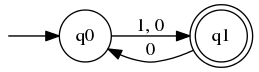
\includegraphics[scale=0.5]{ejd}
    %%\caption{Ejemplo sencillo}
\end{figure}

\noindent 
y queremos calcular su intersección con si mismo, se va a generar un estado $(q^1_0, q^2_1)$ que
correspondería a ``el primer autómata está en el estado 0 y el segundo en el estado 1'', cosa que
nunca puede ocurrir.

Para corregir esto, la definición del conjunto de estados en la intersección pasó a ser

$$
\{(q^1_i, q^2_j) / (q^1_i, q^2_j) \in Q_1 \times Q_2 \wedge \exists \alpha \in \Sigma^* / \delta_1^*(q^1_0, \alpha) = q^1_i \wedge  \delta_2^*(q^2_0, \alpha) = q^2_j \}
$$

Dicho esto, la implementación más sencilla es construír la primer versión y luego eliminar los nodos
sobrantes, es decir, aquellos a los que no se llega partiendo del nodo inicial.  En el ejemplo, los
únicos nodos que quedarían son $(q^1_0, q^2_0)$ y $(q^1_1, q^2_1)$.  Al resultado de esta
construcción se le aplicó la minimización desarrollada en el ejercicio a.

La otra dificultad, como mencionamos, fue un ejemplo mal interpretado.  La intersección entre ``las
cadenas que empiezan con 010'' y ``las cadenas que terminan con 010'' no es ``la cadena
\texttt{'010'}'' sino ``las cadenas que empiezan y terminan con 010'', y sin embargo eso fue lo que
intentamos obtener como salida del algoritmo durante varias horas.  Una vez resuelto el problema
mental, quedó este ejemplo como uno de los tests, junto al caso evidente de la intersección de un
autómata con si mismo que, efectivamente, genera el mismo autómata (usando el autómata del ejemplo)
y la de dos autómatas cuya intersección es vacía, o mejor dicho dos autómatas que aceptan lenguajes
cuya intersección es vacía.

Para esta reentrega se eliminó la excepción que impedía que se calculara la intersección de dos
autómatas con alfabetos distintos.
\section*{Ejercicio e: Complemento de un autómata}
El complemento de dos autómatas es más sencillo de definir: Dado $M = \langle Q, \Sigma, q0, \delta, F \rangle$, con su estado trampa $qT$, el complemento es $M^c = \langle Q, \Sigma, q0, \delta, Q - F \rangle$, y el código simplemente hace eso: define un nuevo autómata.  Apenas tiene un test sencillo.

\section*{Ejercicio f: Equivalencia de autómatas}

En este ejercicio explotamos el teorema 4.26 del \Hopcroft,  según el cual dado un autómata $A$ y su minimización $M$, construída según el algoritmo que estamos usando, entonces $M$ tiene menos estados que cualquier autómata determinístico equivalente a $A$.  Por lo que para decidir si dos autómatas son equivalentes:

\begin{itemize}
\item Minimizamos los dos autómatas
\item Con un DFS recorremos determinísticamente el automata y renombramos los estados según ese orden.
\item Verificamos si para cada estado del primer autómata, existe otro del mismo nombre y con tienen las mismas transiciones.
\end{itemize}

Para este ejercicio implementamos únicamente un unit test con el ejemplo que aparece en el libro.


\bibliographystyle{plain}
\bibliography{references}
\end{document}
